\section{\sysname : Design and Implementation}\label{sec:design}
 We now discuss the design and implementation of \sysname{} --- a system that provides high throughput with predictable tail latency via two key techniques -- \chunking and \hbatch.
 

\begin{figure*}[t!]
    \centering
        \begin{subfigure}[b]{\linewidth}
        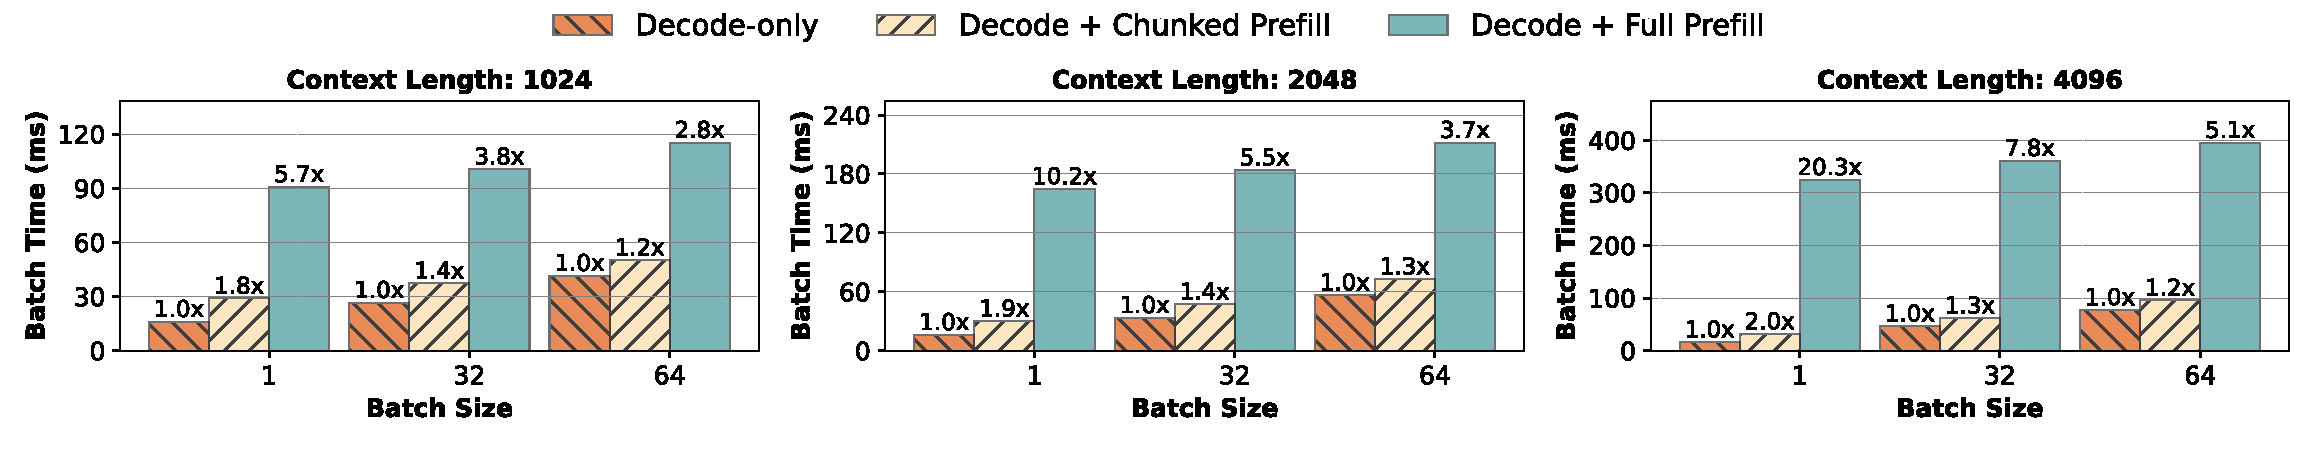
\includegraphics[width=\linewidth]{figures/piggybacking_cost_mistral_7b_1.pdf}
        \caption{Mistral-7B on one A100s with token budget of 256.}
        \label{fig:motivation:incrementalcost:mistral}
    \end{subfigure}
    \\
    \begin{subfigure}[b]{\linewidth}
        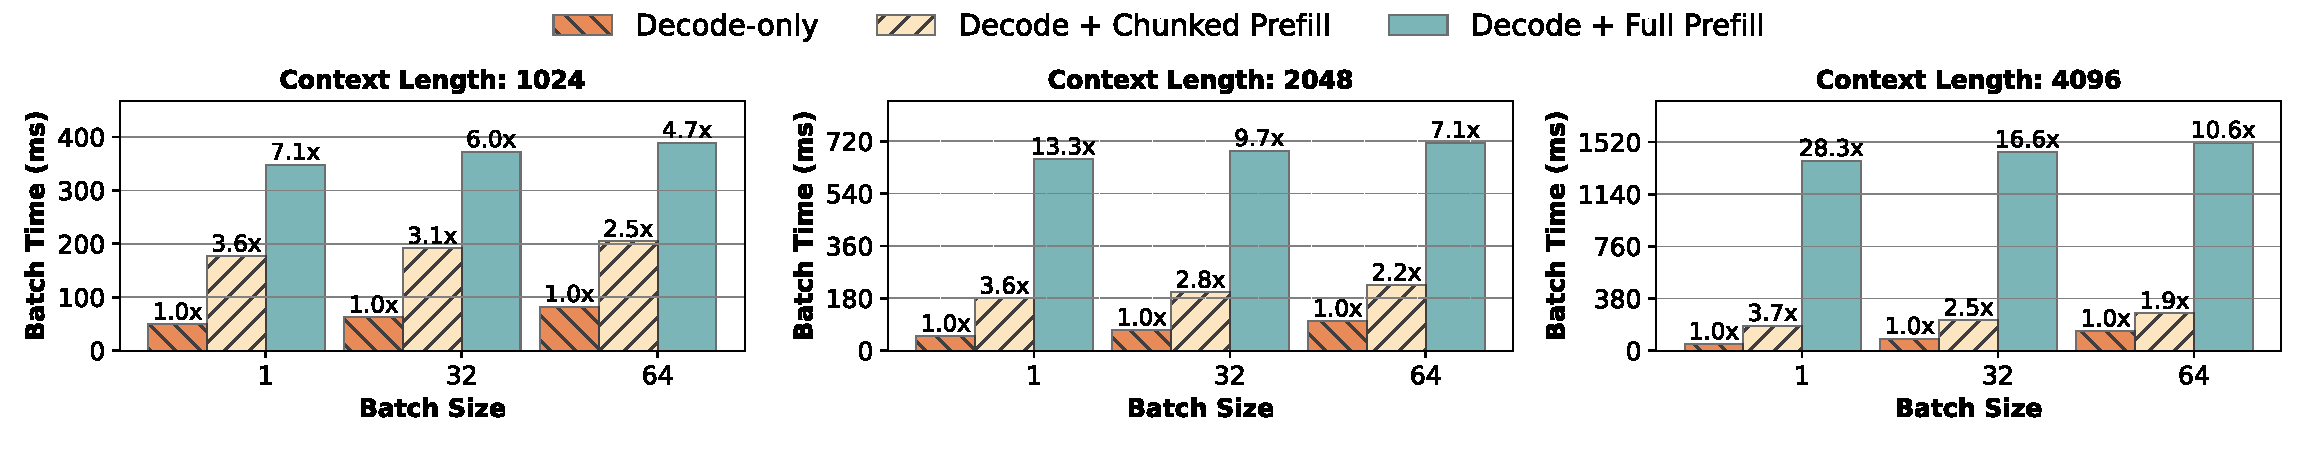
\includegraphics[width=\linewidth]{figures/piggybacking_cost_llama_70b_1.pdf}
        \caption{\llamaL on four A100s with token budget of 512.}
        \label{fig:motivation:incrementalcost:llama}
    \end{subfigure}

    \caption{The incremental cost of coalescing prefills with decode batches. We consider two batching schemes -- (i) Decode + Full Prefill represents the hybrid batching of Orca wherein the entire prefill is executed in a single iteration along with ongoing decodes. (ii) Decode + Chunked Prefill represents \sysname wherein prefills are chunked before being coalesced with ongoing decodes with a fixed token budget. \sysname processes prefill tokens with much lower impact on the latency of decodes. Further, the relative impact of \sysname on latency reduces with higher decode batch size and context lengths.}
        \label{fig:motivation:incrementalcost}
\end{figure*}





\subsection{Chunked-prefills}
\label{sec-design-chunkedprefill}

As we show in \autoref{sec:analysis:throughput}, decode batches are heavily memory bound with low arithmetic intensity. This slack in arithmetic intensity presents an opportunity to piggyback additional computation in decode batches. Naively, this can be done by creating hybrid batches which combine the memory bound decodes along with compute bound prefills. However, in many practical scenarios, input prompts contain several thousand tokens on average \eg \autoref{table:eval:datasets} shows that the median prompt size in \sharegpt and \arxivsum datasets is 1730 and 7059 respectively. Combining these long prefills with decode iterations would lead to high TBT latency.

To tackle this challenge, we present a technique called \chunking which allows computing large prefills in small chunks across several iterations. \Chunking is a prefill splitting mechanism hinged on two key insights. First, as discussed in~\autoref{sec:analysis:throughput}, a prefill request with modest sequence length can effectively saturate GPU compute. For example, in~\autoref{fig:motivation:op-wise-time}, prefill throughput starts saturating around sequence length of 512 tokens. Second, in many practical scenarios, input prompts contain several thousand tokens on average (\autoref{table:eval:datasets}). This provides an opportunity to break large prefill requests into smaller units of compute which are still large enough to saturate GPU compute. In \sysname, we leverage this mechanism to form batches with appropriate number of tokens such that we can utilize the compute potential in decode batches without violating the TBT SLO.

\algrenewcommand\algorithmicindent{1em}
\begin{algorithm}[t!]
\caption{\Hbatch with \sysname.  First the batch is filled with with ongoing decode tokens (lines 6-8) and optionally one prefill chunk from ongoing (lines 10-12). Finally, new requests are added (lines 13-20) within the token budget so as to maximize throughput with minimal latency impact on the TBT of delaying the ongoing decodes.}
\label{alg:stall_free}
\begin{algorithmic}[1]
\State \textbf{Input:} $T_{max}$, Application TBT SLO.
\State Initialize \textit{token\_budget}, $\tau$ $\leftarrow$ compute\_token\_buget($T_{max}$)
\State Initialize \textit{batch\_num\_tokens}, $n_t$ $\leftarrow$ 0
\State Initialize current batch $B \leftarrow \emptyset$

\While{True}
    \For{$R$ in $B$}
        \If{is\_prefill\_complete($R$)} %
            \State $n_t \leftarrow n_t + 1$
        \EndIf
    \EndFor
    
    \For{$R$ in $B$}
        \If{not is\_prefill\_complete($R$)} %
            \State $c \leftarrow$  get\_next\_chunk\_size($R$, $\tau$, $n_t$)
            \State $n_t \leftarrow n_t + c$
        \EndIf
    \EndFor
    
    \State $R_{new} \leftarrow$ get\_next\_request()

    \While {can\_allocate\_request($R_{new}$)  $ \land$ $n_t$ < $\tau$} %
        \State $ c \leftarrow$  get\_next\_chunk\_size($R_{new}$, $\tau$, $n_t$)
        
        \If{$c$ > 0}
            \State $n_t \leftarrow n_t + c$
            \State $B \leftarrow R_{new}$ 
        \Else
            \State break
        \EndIf
    \EndWhile

    \State
    \State process\_hybrid\_batch($B$)
    \State $B \leftarrow$ filter\_finished\_requests($B$)
    \State $n_t \leftarrow 0$
\EndWhile
\end{algorithmic}
\end{algorithm}



\subsection{\Hbatch}



The \sysname scheduler is an iteration-level scheduler that leverages \chunking and coalescing of prefills and decodes to improve throughput while minimizing latency.

Unlike Orca and vLLM which stall existing decodes to execute prefills, \sysname leverages the arithmetic intensity slack in decode iterations to execute prefills without delaying the execution of decode requests in the system. We call this approach \hbatch (\autoref{alg:stall_free}). \sysname first calculates the budget of maximum number of tokens that can be executed in a batch based on user specified SLO. We describe the considerations involved in determining this token budget in depth in \autoref{section:howtopickachunksize}. In every scheduling iteration, we first pack all the running decodes in the next batch (lines 6-8 in \autoref{alg:stall_free}). After that, we include any partially completed prefill (lines 9-12). Only after all the running requests have been accommodated, we admit new requests (lines 13-20). When adding prefill requests to the batch, we compute the maximum chunk size that can be accommodated within the leftover token budget for that batch (lines 11, 15). By restricting the computational load in every iteration, \hbatch ensures that decodes never experience a generation stall due to a co-running prefill chunk.  We compare the latency for hybrid batches with and without chunked prefills in \autoref{fig:motivation:incrementalcost}. Naive hybrid batching leads to dramatic increase of up to 28.3\myx in the TBT latency compared to a decode-only batch. In contrast, \sysname provides a much tighter bound on latency with chunking.

\autoref{fig:motivation:generationstalls} shows the scheduling policy of \sysname in action, for the same example used in~\autoref{sec:latencyandstalls}. The first iteration is decode-only as there are no prefills to be computed. However, after a new request C enters the system, \sysname first splits the prefill of C into two chunks and schedules them in subsequent iterations. At the same time, with \hbatch, it coalesces the chunked prefills with ongoing decodes of A and B. This way, \sysname stalls neither decodes nor prefills unlike existing systems, allowing \sysname to be largely free of latency spikes in TBT without compromising throughput. Furthermore, \hbatch combined with \chunking also ensures uniform compute hybrid batches in most cases, which helps reduce bubbles when using pipeline parallelism, thereby enabling efficient and scalable deployments.

\subsection{Determining Token Budget}
\label{section:howtopickachunksize}

The token budget is determined based on two competing factors --- TBT SLO requirement and \chunking overhead. From a TBT minimization point of view, a smaller token budget is preferable because iterations with fewer prefill tokens have lower latency. However, smaller token budget can result in excessive chunking of prefills resulting in overheads due to 1) lower GPU utilization and 2) repeated KV-cache access in the attention operation which we discuss below.

During the computation of \chunking, the attention operation for every chunk of a prompt needs to access the KV-cache of \textit{all} prior chunks of the same prompt. This results in increased memory reads from the GPU HBM even though the computational cost is unchanged. For example, if a prefill sequence is split into $N$ chunks, then the first chunk's KV-cache is loaded $N-1$ times, the second chunk's KV-cache is loaded $N-2$ times, and so on. However, we find that even at small chunk sizes attention prefill operation is compute bound operation. In practice, there can be small overhead associated with chunking due to fixed overheads of kernel launch, etc. We present a detailed study of the overheads of \chunking in \autoref{sec-eval-ablation}.


Thus, one needs to take into account the trade-offs between prefill overhead and decode latency while determining the token budget. This can be handled with a one-time profiling of batches with different number of tokens and setting the token budget to maximum number of tokens that can be packed in a batch without violating TBT SLO. 

Another factor that influences the choice of token budget is the \textit{tile-quantization} effect~\cite{tile-quantization}. GPUs compute matmuls by partitioning the given matrices into tiles and assigning them to different thread blocks for parallel computation. Here, each thread block refers to a group of GPU threads and computes the same number of arithmetic operations. Therefore, matmuls achieve maximum GPU utilization when the matrix dimensions are divisible by the tile size.  Otherwise, due to \textit{tile-quantization}, some thread blocks perform extraneous computation~\cite{tile-quantization}. We observe that tile-quantization can dramatically increase prefill computation time \eg in some cases, using chunk size of 257 can increase prefill time by 32\% compared to that with chunk size 256.

Finally, when using pipeline parallelism the effect of token budget on pipeline bubbles should also be taken into account. Larger chunks lead to higher inter-batch runtime variations that result in pipeline bubbles which results in lower overall system throughput. On the other hand, picking a very small token budget can lead to higher overhead due to lower arithmetic intensity and other fixed overheads.

Therefore, selecting a suitable token budget is a complex decision which depends on the desired TBT SLO, parallelism configuration, and specific hardware properties. We leverage Vidur~\cite{vidur}, a LLM inference profiler and simulator to determine the token budget that maximizes system capacity under specific deployment scenario.



\subsection{Implementation} We implement \sysname on top of the open-source implementation of vLLM \cite{vllmsosp, vLLM:github}. %
We added support for paged chunk prefill using FlashAttention v2 \cite{flashattention2} and FlashInfer \cite{flashinfer} kernels. We use FlashAttention backend for all the evaluations in this paper due to its support for wider set of models. We also extend the base vLLM codebase to support various scheduling policies, chunked prefills, pipeline parallelism and an extensive telemetry system. We use NCCL \cite{nccl} for both pipeline and tensor parallel communication.
Source code for the project is available at ~\href{https://github.com/microsoft/sarathi-serve}{https://github.com/microsoft/sarathi-serve}. %


\begin{table}[tb!]
\centering
\setlength{\tabcolsep}{2pt}
\scalebox{0.78}{
\begin{tabular}{r|c|c|c}
\multirow{2}{*}{\textbf{Model}} & \textbf{Attention} & \textbf{GPU} & \textbf{Memory} \\
& \textbf{Mechanism} & \textbf{Configuration} & \textbf{Total (per-GPU)} \\ \toprule
Mistral-7B & GQA-SW & 1 A100 & 80GB (80GB) \\
Yi-34B & GQA & 2 A100s (TP2) & 160GB (80GB)\\
LLaMA2-70B & GQA & 8 A40s (TP4-PP2) & 384GB (48GB) \\
Falcon-180B & GQA & 4 A100s\myx{}2 nodes (TP4-PP2) & 640GB (80GB) \\
\bottomrule
\end{tabular}}
\caption{Models and GPU configurations (GQA: grouped-query attention, SW: sliding window).}
\label{table:eval:models}
\end{table}
